% Lecture Template for ME3001-001-Tristan Hill - Spring 2017 - Fall 2017
% 
% Mechanical Engineering Analysis with MATLAB
%
% Systems of Linear Equations - Lecture 2
%


% Document settings
\documentclass[11pt]{article}
\usepackage[margin=1in]{geometry}
\usepackage[pdftex]{graphicx}
\usepackage{multirow}
\usepackage{setspace}
\usepackage{hyperref}
\usepackage{color,soul}
\usepackage{fancyvrb}
\usepackage{framed}
\usepackage{wasysym}
\usepackage{multicol}

\pagestyle{plain}
\setlength\parindent{0pt}
\hypersetup{
    bookmarks=true,         % show bookmarks bar?
    unicode=false,          % non-Latin characters in Acrobat’s bookmarks
    pdftoolbar=true,        % show Acrobat’s toolbar?
    pdfmenubar=true,        % show Acrobat’s menu?
    pdffitwindow=false,     % window fit to page when opened
    pdfstartview={FitH},    % fits the width of the page to the window
    pdftitle={My title},    % title
    pdfauthor={Author},     % author
    pdfsubject={Subject},   % subject of the document
    pdfcreator={Creator},   % creator of the document
    pdfproducer={Producer}, % producer of the document
    pdfkeywords={keyword1} {key2} {key3}, % list of keywords
    pdfnewwindow=true,      % links in new window
    colorlinks=true,       % false: boxed links; true: colored links
    linkcolor=red,          % color of internal links (change box color with linkbordercolor)
    citecolor=green,        % color of links to bibliography
    filecolor=magenta,      % color of file links
    urlcolor=blue           % color of external links
}

% assignment number 
\newcommand{\NUM}{2} 
\newcommand{\VSpaceSize}{2mm} 
\newcommand{\HSpaceSize}{2mm} 

\definecolor{mygray}{rgb}{.6, .6, .6}

\setulcolor{red} 
\setstcolor{green} 
\sethlcolor{mygray} 

\begin{document}

\textbf{ \LARGE ME 3001 Lecture, Systems of Linear Equations} \\\\
\textbf{ \LARGE A Brief Review of Linear Algebra in MATLAB} \\

\begin{itemize}

\item \textbf{\LARGE General Form of  A Linear System (review)}
	\Large
	\begin{itemize}
		\item The System of Equations \\ \\
		  \scalebox{1.2}{$a_{11} x_1 + a_{12} x_{2} + ... + a_{1n} x_n = b_1 $} \\
		  \scalebox{1.2}{$a_{21} x_1 + a_{22} x_{2} + ... + a_{2n} x_n = b_2 $} \\
		  \scalebox{1.2}{$\hspace{20mm}.$}\\
		  \scalebox{1.2}{$\hspace{20mm}.$}\\
		  \scalebox{1.2}{$\hspace{20mm}.$}\\		
		  \scalebox{1.2}{$a_{n1} x_1 + a_{n2} x_{2} + ... + a_{nn} x_n = b_n $} \\\vspace{20mm}		
		  
		 \item The System in Matrix Form 	\\\\
\scalebox{1.2}{$	 	
 \left( \begin{array}{cccc}
a_{11} & a_{12} & ...& a_{1n} \\
a_{21} & a_{22} & ...& a_{2n} \\
&.&&\\
&.&&\\
a_{n1} & a_{n2} & ...& a_{nn}\end{array} \right) \times \left[ \begin{array}{c}
x_1 \\
x_2 \\
.\\
.\\
x_n \end{array} \right] = \left[ \begin{array}{c}
b_1 \\
b_2 \\
.\\
.\\
b_n \end{array} \right] 
$}\\\\

 \item A common mistake 
\end{itemize}

\newpage
%\item \textbf{\LARGE What is Matrix Multiplication}	
%\begin{itemize}
%		\item Consider 2 conformable matrices $F$ and $G$ with elements $f_{ij}$ and $g_{ij}$. 
%		 \item Matrix Multiplication gives the product matrix $E$ with elements $e_{ij}$.  \\ \vspace{5mm}
%		 
%		 	 \scalebox{1.2}{ $E = F \times G \hspace{20mm} e_{ij}=\Sigma_{k=1}^n f_{ik}\times g_{kj}$} \\ \vspace{20mm}
%		 
%		 \item Lets do an example with a few small matrices. \\
%		 
%		 \scalebox{1.2}{$
%		  \left[ \begin{array}{cc}
%e_{11} & e_{12}  \\
%e_{21} & e_{22}  \end{array} \right]=	 	
% \left[ \begin{array}{ccc}
%f_{11} & f_{12} & f_{13} \\
%f_{21} & f_{22} & f_{23} \end{array} \right] \times \left[ \begin{array}{cc}
%g_{11}&g_{12} \\
%g_{21}&g_{22} \\
%g_{31}&g_{32} \end{array} \right] 
%$} 
%
%		 
%		 \vspace{20mm}
%		 
%		 \item A closer look at E \\ \vspace{10mm}
%		 
%\scalebox{1.2}{$
%		  \left[ \begin{array}{cc}
%		e_{11} & e_{12}  \\
%		& \\ 
%		e_{21} & e_{22}  \end{array}	\right]=\left[ \begin{array}{c|c}
%		f_{11}g_{11}+f_{12}g_{21}+f_{13}g_{31} & f_{11}g_{12}+f_{12}g_{22}+f_{13}g_{32}  \\
%		& \\ 
%		f_{21}g_{11}+f_{22}g_{21}+f_{23}g_{31} & f_{21}g_{12}+f_{22}g_{22}+f_{23}g_{32}  \end{array}	\right]
%		 $} \\\\
%		 
%	
%
%	\item So what is n ? 
%	\end{itemize}
%\newpage	
%	\item \textbf{\LARGE A Programming Exercise - Matrix Multiplication}\\	
%		\begin{itemize}
%		
%		\item  \scalebox{1.2}{ $e_{ij}=\Sigma_{k=1}^n f_{ik}\times g_{kj}$} \\
%		\item What does that equation mean? \\
%		\item How can we write a {\it General Solution Technique}?
%		\end{itemize}
%\newpage
%
\item \textbf{\LARGE A Mechanical Engineering Example}\\	
		
		As a group we are going to setup and solve a small statics problem. \\
		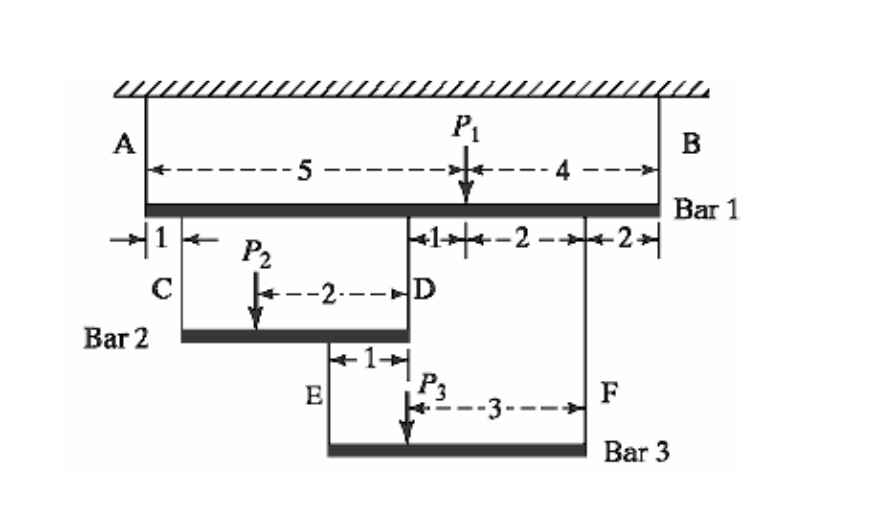
\includegraphics[scale=.75]{lecture1_fig1.png}\\
		{\Large
		\begin{itemize}
		 \item \textbf{bar 1} 	\\\\
		 \newpage
		  \item \textbf{bar 2}	\\ \vspace{80 mm}
		   \item \textbf{bar 3} 	\\\\
		\end{itemize} }
\newpage

\item \textbf{\LARGE A Mechanical Engineering Example (continued)}\\			

		

		




\newpage 

	\item \textbf{ \LARGE REMINDER - Homework 2 has been Posted.} \\
	 \item \textbf{ \LARGE REMINDER - Homework 2 is due Wed. Feb. 8} \\
	\item \textbf{ \LARGE REMINDER - MATLAB script from today's lecture will be posted on ilearn. } \\

\end{itemize}


	

\end{document}



